\chapter{Data Processing}
\label{sec:data_processing}

In this chapter, we discuss the data processing steps that are required to prepare the data for the model development process. Firstly, we address different session parameters and how they might influence the data. Secondly, we explain the data acquisition process and how the data is stored in files such that it can be used in the future. Thirdly, we discuss the data population process in which the human pose data is extracted from the raw data. To ensure the quality of the dataset we then evaluate the data by filtering invalid skeletons and marking data points as valid or invalid. Finally, we discuss the data augmentation process in which the data is augmented to increase the size of the dataset.

\section{Stream pre-processing}
\label{sec:stream_pre_processing}

To get the best possible results we need to make sure that the cameras are set up in exactly the intended way. 

\subsection{Multiple Cameras}

We use multiple cameras to increase the accuracy of the results. We use two cameras to record the same scene from two different angles. This way we can compare the results from the two cameras and make sure that the results are consistent. We also use multiple cameras to record the same scene from different heights and angles.

\textit{\textbf{UNSURE} Should I write about it if Im not going to do it? Its quite interesting how the synchronisation might work and how the pointclouds can be synchronised. I already did a lot of research on it but if Im not going to implement it then this might not be the best point to do it.}

\subsection{Recording session set-up}

We consider different environmental setups to increase the significance of the results. The following session parameters are considered:

\subsubsection{Lighting}

RGBD cameras function with infrared light therefore is the lighting of a scene essential. We found that direct sunlight interferes with some RGBD cameras more than others based on the infrared range that is used. Since the exact sunlighting is not controllable we choose to make it as optimal as possible to improve reproducibility. Therefore, we choose a room with no sunlight but we do include artificial light to reduce any damage that might occur to visibility issues.

\subsubsection{Relative Camera Position}

At SilverFit, cameras are attached above a screen at a height of $180 cm$ facing downward at around $20\deg$. To form a more general model, we will experiment with different setups and angles. We experiment with six different setups in total. Three setups from different angles ($20\deg, 0\deg, 340\deg$) at two different heights ($180cm$, $120cm$). The different setups can be seen in figure TODO.

\textit{\textbf{TODO} Add figure with different setups.}

\textit{
  \textbf{UNSURE} We Develop a functionality that lets us determine the exact height and orientation of the camera. We do this by detecting the floor and thereby calculating the height of the camera and the angle at which it is pointing downward. We can also detect if the camera is not completely straight and therefore might influence the results.
}

\subsubsection{Sitting or standing}

From experience, we know that detecting the joints correctly is influenced by the position of the participant. This is especially true for the difference between a sitting and a standing patient. Human pose detection is in general more reliable if the patient is standing, due to reduced occlusion. We record each scenario sitting and standing.

\subsubsection{Clothing and ankle and wrist attachments}

Clothing can have a similar effect on the efficacy of HPE as lighting. If the participant is wearing black pants infrared light will be absorbed rather than reflected leading to 'blind spots' in the legs. Since the legs are already more unreliable than the rest of the body, these blind spots can negatively affect HPE. 

Since SilverFit develops games for rehabilitation, the supervising physiotherapist might choose to attach weights to the ankles and/or wrists to increase the effectiveness of the exercise. We therefore also include attached and held weights to simulate difficult situations.

\subsubsection{Background}

The background of the scene can have a significant effect on the results. We, therefore, record the same scenario with and without a visible background, i.e. a wall is behind the participant or there is no wall within the maximum sensor range ($6m$).

\subsubsection{Crampedness of the Environment}

The Crampedness of the scene increases the number of false positives of HPE. We, therefore, record the same scenario with and without clutter. We consider clutter to be any object that is not a part of the participant's body. However, clutter is quite objective and therefore we will not be able to define it in a universally applicable way. 

\subsubsection{Distance to the camera}

Games developed by SilverFit have a calibration step where the participant is asked to stand at a certain distance from the camera. We, therefore, record the scenario at that specific distance. This ensures that noise introduced by the depth sensor has little effect on the results. The participant is positioned 2 meters away from the camera. \textit{UNSURE, ask someone at SilverFit}.



\section{Data acquisition}
\label{sec:data_acquisition}

The second phase of the pipeline is data acquisition. After we have set up the camera according to the session parameters we can start recording. We set a timer for $30s$ and record the RGB and Depth streams from the camera. We also record the camera intrinsics, which we will use to recreate the point cloud at a later stage. We record the data in a folder structure that is defined by the session parameters.

\subsection{Data format}

An important part of data acquisition is the description of the way the data is stored in the file system. This is essential for any future use of the data and therefore we need to make sure that the data is stored in a way that is easy to understand and easy to use. We store in general two to five files per session depending on the camera configuration. 

\subsubsection{Session Metadata}

Every session contains a "\texttt{SESSION\_NAME.json}" file that contains the session parameters and camera metadata. The session name is automatically generated based on the starting time of the session, this way we can make sure that the session name is unique every time and we can also have an idea of which recording is the most recent without looking at the contents of the file.

\paragraph{Camera metadata}

The camera metadata contains the camera intrinsics, which we will use to recreate the point cloud at a later stage. The camera intrinsics are the field of view of the depth camera in the horizontal and vertical direction, and the principal point in the horizontal and vertical direction. The field of view is the angle between the optical axis and the image plane. The principal point is the point in the image where the optical axis of the camera intersects the image plane. The principal point and the field of view are explained in Figure \ref{fig:pinhole_camera_model}.

\begin{figure}[ht]
  \centering
  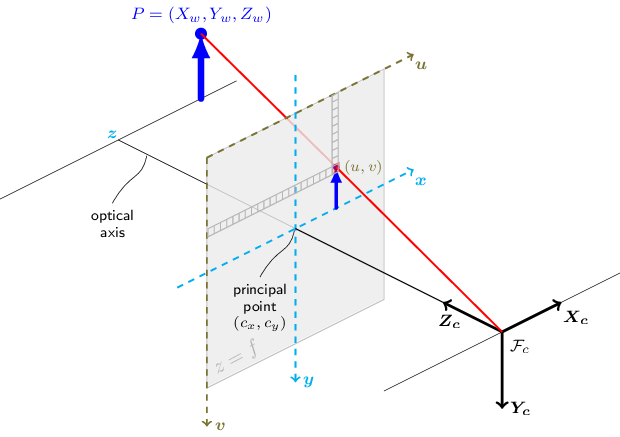
\includegraphics[width=.9\textwidth]{figures/CameraCalibration/pinhole_camera_model.png}
  \caption[Pinhole camera model]{The pinhole camera model showing the principal point. The principal point is the point where the optical axis intersects the image plane. The field of view is the angle between the optical axis and the image plane.}
  \label{fig:pinhole_camera_model}
\end{figure}

\paragraph{Camera orientation}

Additionally, to the camera intrinsics we store the relative rotation and translation between the cameras if multiple cameras are used. The rotation and translation are stored as Euler angles\footnote{Technically we are storing the rotation with the Tait–Bryan notation, i.e. x-y-z or yaw-pitch-roll, rather than the classic Euler notation. However, the name Euler angle is more commonly used and understood.} and a vector respectively \cite{euler1776formulae}. The rotation is the rotation of the camera relative to the second camera in the system. The translation is the translation of the camera concerning the second camera in the system.

\paragraph{Session parameters}

The session parameters are the same as the ones defined in the section "Stream pre-processing". The user enters the session parameters before starting the recording. Most of the parameters are boolean values that indicate whether the user is sitting, wearing dark clothing, etc. The height and angle parameters are the height of the camera to the floor and the angle of the camera relative to the orientation of the user as explained in the previous section.

An example of the Session metadata can be seen in Listing \ref{lst:session_metadata}.

\begin{lstlisting}[language=json,
                   firstnumber=1,
                   caption={[Example of session metadata]{Example of the Session metadata with a single Realsense Camera which was recorded for 40 seconds at around 30 frames per second resulting in 1200 frames. Some values have been changed to increase readability.}},
                   label={lst:session_metadata}]
{
  "Cameras" : 
  [
    {
      "Cx" : 314.26,
      "Cy" : 239.46,
      "FileName" : "Session_2023-01-30T09.21.34_Realsense_Camera_0.bag",
      "Fx" : 459.77,
      "Fy" : 459.83,
      "MeterPerUnit" : 0.00025,
      "Name" : "Realsense Camera 0",
      "Type" : "Realsense"
    }
  ],
  "DurationInSec": 40.0,
  "Name": "Session 2023-01-30T09:21:34",
  "RecordedFrames": 1200,
  "Rotation": {
      "Roll": 0.0,
      "Pitch": 0.0,
      "Yaw": 0.0
  },
  "Translation": {
      "X": 0.0,
      "Y": 0.0,
      "Z": 0.0
  },
  "Session Parameters": {
    "Sitting": true,
    "Background close": true,
    "Cramped": false,
    "Dark Clothing": true,
    "Holding Weight": false,
    "Ankle Weight": false,
    "Height": 1.8,
    "Angle": 20.0
  }
}
\end{lstlisting}

\subsubsection{Realsense Cameras}

We record Realsense Cameras using the librealsense SDK provided by Intel. Using the SDK we have access to the Hight-Level Pipeline API which allows us to stream the camera feed and access the camera intrinsics. This High-Level Pipeline API allows us to record the RGB and Depth streams from the Realsense camera. The SDK automatically synchronises the Depth and RGB stream as well as the motion sensors, which we do not use since our camera is static. The librealsense SDK is available on GitHub\footnote{\url{https://github.com/IntelRealSense/librealsense}}.

The Recordings are stored in a ROS bag file. A ROS bag file is a file format for storing ROS messages. The ROS bag file format is a container format that stores multiple messages in a single file. The ROS bag file format is described in detail in the ROS wiki\footnote{\url{http://wiki.ros.org/Bags}}. The ROS bag file format is a container format that stores multiple messages in a single file. In our case, the important messages are the camera intrinsics, which allow us to create a virtual Realsense Camera from the recording, the RGB stream, and the Depth stream. However, other messages are also stored and can be accessed using the ROS Bag API\footnote{\url{http://wiki.ros.org/rosbag/Code\%20API}}.

\subsubsection{Orbbecc Astra Cameras}

To read the depth stream of the Orbbecc Astra camera we use the OpenNI2 API\footnote{\url{https://structure.io/openni}}. The OpenNI2 API is a cross-platform API that allows us to access the depth stream of the Orbbecc Astra camera. The OpenNI API is no longer being developed by PrimeSense and has been renamed to OpenNI2 to avoid confusion with the OpenNI API. The OpenNI2 API is available on GitHub\footnote{\url{https://github.com/structureio/OpenNI2}}.

Using the OpenNI2 API we can also record the depth stream to a file. The depth stream is stored as a \texttt{.ONI} file. The \texttt{.ONI} file format is a proprietary format that is not documented. However, the OpenNI2 API provides a \texttt{.ONI} file reader that allows us to access the depth stream.

Sadly, the OpenNI2 API does not provide a way to access the RGB stream. Therefore, we use the OpenNI2 API to access the depth stream and OpenCV to access the RGB stream. The RGB stream is stored as a \texttt{.AVI} file. The \texttt{.AVI} file format is a container format that stores multiple video streams in a single file. The \texttt{.AVI} file format is described in detail in the Microsoft documentation\footnote{\url{https://docs.microsoft.com/en-us/previous-versions/ms779636(v=vs.85)}}. 

\textit{
  \textbf{ISSUE}: currently the playback of the \texttt{.AVI} file is only possible at a specific framerate, which is set at the beginning of the recording session. This poses a substantial issue regarding synchronisation. Shoul I write about this?
}

\subsection{Recording process}

Once the scene is set and the pointclouds have been aligned the user can start the recording. Firstly, there are pre recording settings such as a frame and/or time limit in seconds, which allows accurate time and/or frame constraints to create equal recordings. Secondly, the user can select whether or not to display the pointcloud while recording. This allows the user to see the pointcloud in real-time and adjust the recording accordingly, however, this leads to a substantially reduced framerate\footnote{From 30 FPS, without pointcloud to 15 FPS with pointcloud}. These can be set in the GUI as shown in Figure \ref{fig:recording_gui}. Finally, the user can configure the session parameters described earlier. After the recording has beend started by the user a preconfigured countdown will be started, allowing the user to get into position in time. Once the countdown has finished the recording will start. The recording will stop once the time or frame limit has been reached. The recording will also stop if the user presses the stop button.  

\begin{figure}[ht]
  \centering
  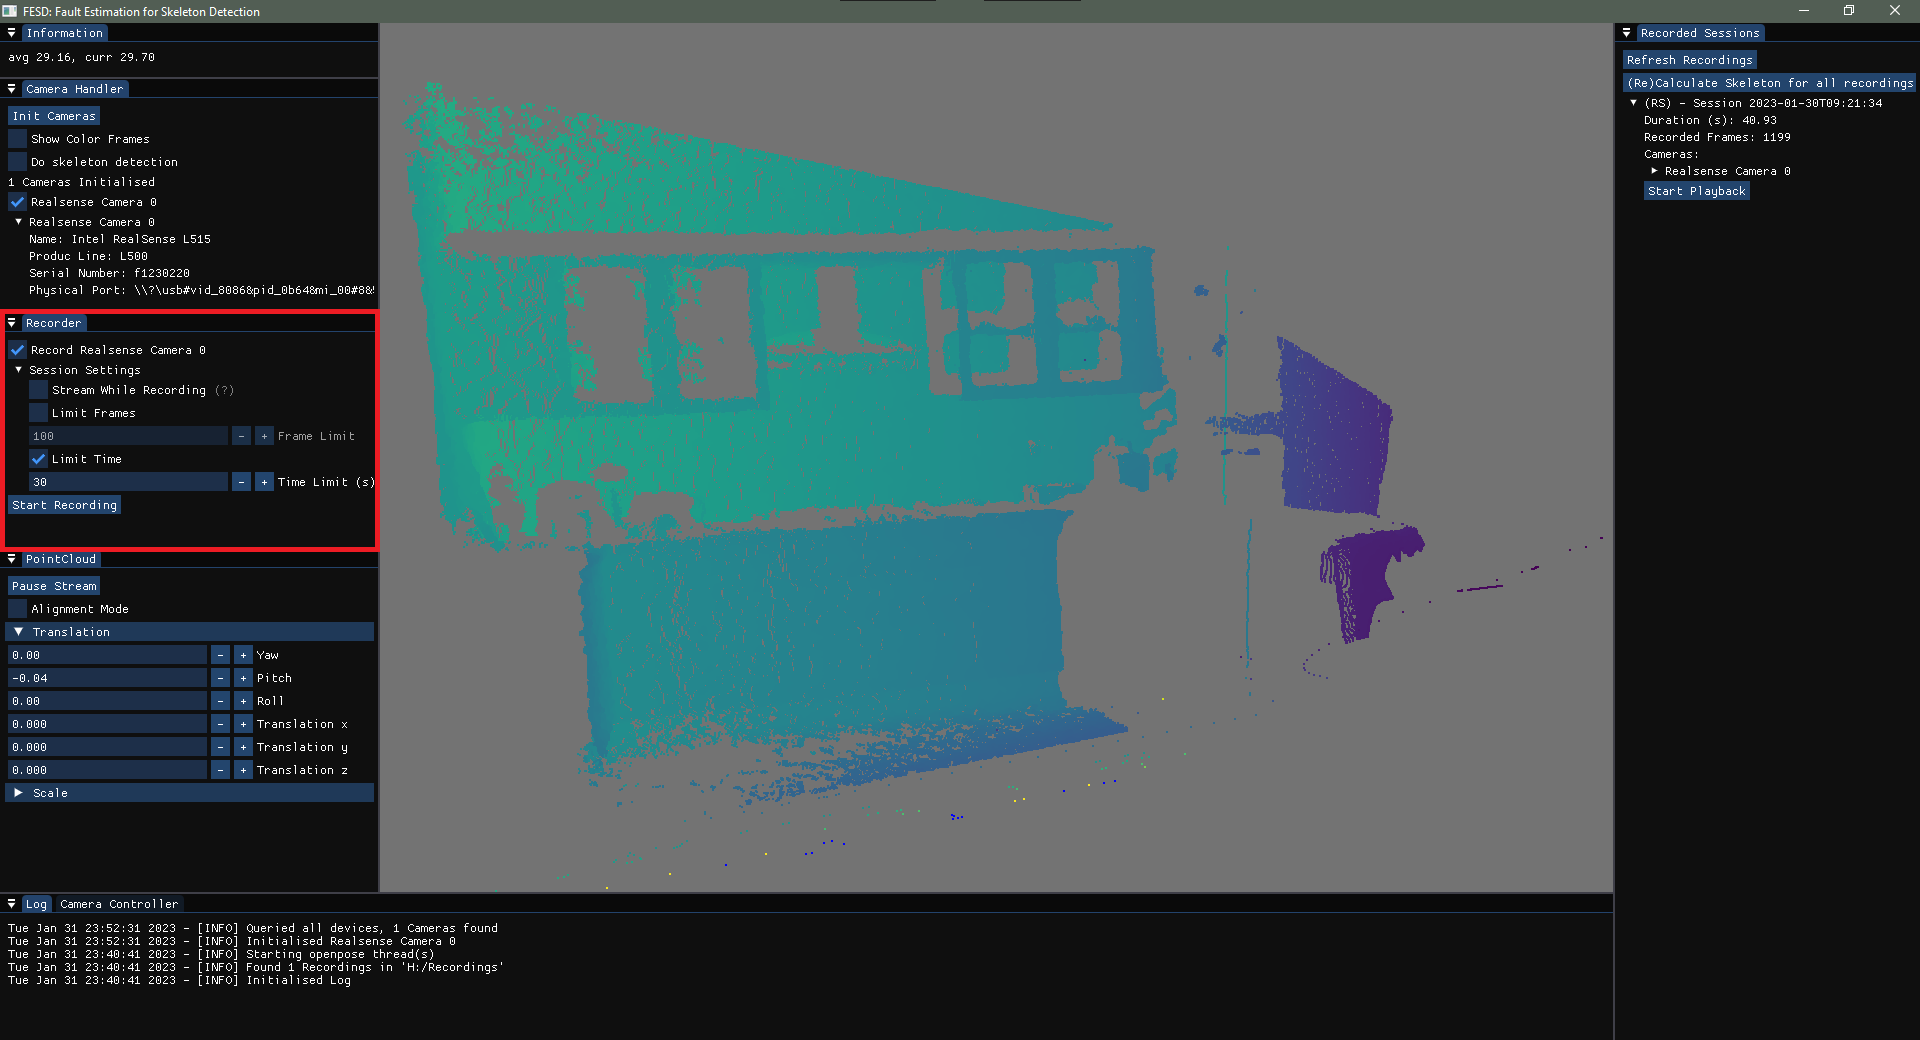
\includegraphics[width=0.8\linewidth]{figures/FESD/recording_gui.png}
  \caption[Recording GUI marked in Red]{Recording GUI marked in Red. The user can set the recording parameters here such as the time and frame limits and whether or not the .}
  \label{fig:recording_gui}
\end{figure}
\section{Data population}
\label{sec:data_population}

\textit{\textbf{JUST AS REFERENC} To achieve the highest framerate, $REPLACE_WE$ calculate the skeleton based on the recorded data and add it to the dataset in a separate step. The RGB stream is used to create the dataset for the skeleton detection and the depth stream is used to create the point clouds for the calculation of global skeleton points. $REPLACE_WE$ store both the local 2D coordinates in accordance with the image used for the skeleton detection, as well as the global 3D coordinates based on the aligned point clouds. Additionally, OpenPose provides $REPLACE_US$ with a confidence score for each joint.}

\textit{\textbf{DECISION} I decided to switch to NuiTrack, it is closer to silverfit and I think a better choice. Openpose poses more problems than it solves}

\textit{\textbf{TODO} Explain what is meant by Data Population (skeleton detection)}.

\subsection{Human Pose Estimators}

\subsubsection{OpenPose}

\textit{\textbf{TODO} Give rough overview of Openpose and how the projection might have worked}.

\subsubsection{NuiTrack}

To utilise skeleton data, as well as the human silhouette in their games, SilverFit utilises the NuiTrack SDK.  \textit{\textbf{TODO} Explain what NuiTrack is and does and how it works}.

\subsection{Human Pose Estimation}

Human pose estimation is not trivial in terms of resource usage. Calculating the human pose while recording would mean a significant reduction of the recorded frames. Therefore, $REPLACE_WE$ calculate the skeleton seperatly for each frame of the recording.

The skeletons is stored ... \textit{\textbf{TODO} Explain how the skeleton is stored}.
\section{Data Evaluation}
\label{sec:data_evaluation}

Next, we evaluate the recorded data and especially the detected skeleton. We focus specifically on the joints with a low confidence value. 

We discard frames with lacking pose data from the training dataset, they are not usable to train a model. We might still use it for the testing phase. If we notice that the dataset is getting too small, we might re-record some sessions.

\textit{\textbf{QUESTION} Should I discard frames with limited joints?}

Additionally, while recording multiple people might be wrongly detected. However, in our experiments we only consider single person recordings. Therefore, we can discard other people from the data.

The pseudo code for the data evaluation process can be seen in Listing \ref{lst:data_eval}. Most of the checks mentioned, such as \texttt{selectInvalidPeople} in Line 9 or \texttt{checkJointValidity} in Line 14 happen manually. However, the data processing is done automatically by the code to redue human error.

\begin{lstlisting}[language=python,
                    firstnumber=1,
                    caption={[Pseudo code for data evaluation]{Pseudo code for data evaluation}},
                    label={lst:data_eval}]
  def data_evaluation(recording):
    invalid_frames = []
    for frame in recording:
      if not frame:
        invalid_frames.append(frame)
        continue
      else:
        if len(frame.people) > 1:
          invalid_people = frame.selectInvalidPeople()
          frame.remove(invalid_people)

        for joint in frame.people[0].skeleton:
          if joint.confidence < CONFIDENCE_THRESHOLD:
            checkJointValidity(joint)
    
    if len(invalid_frames) > INVALID_LIMIT:
      return False
    
    recording.replace(invalid_frames, Null)

    return True
\end{lstlisting}

\section{Data Augmentation}
\label{sec:data_augmentation}

Once the data is cleaned and REPLACE_WE filter recordings with too many missing joints, REPLACE_WE can augment the data to simulate a larger amount of data with the ability to create faulty scenarios controlled. One major fault is the seemingly random detachment of the joint to a side. This especially affects the legs and arms, therefore REPLACE_WE will have a bias toward limbs with this augmentation. 

Furthermore, REPLACE_WE randomly move the joints with low confidence. Another fault is the disappearance of joints. REPLACE_WE use the same bias as with the random detachment, i.e. REPLACE_WE take the limb bias, as well as the confidence into consideration.

This phase allows REPLACE_US to create a large amount of data with a controlled amount of faults. This is important since REPLACE_WE want to be able to train a model that can detect faults in the data. The augmented data is stored in a separate file so that REPLACE_WE can use it to train the model and compare it to the original manually checked ground truth.

\textit{\textbf{TODO} Create some screenshots of the augmented data from the different methods.}